\documentclass[12pt]{article}
\usepackage{esqu1}
\pagestyle{fancy}

\lhead{Brandon Lin}
\chead{Differential Equations}
\rhead{Spring 2016}

\begin{document}
\title{Differential Equations}
\author{Brandon Lin\\Stuyvesant High School\\Spring 2016\\Teacher: Mr. Stern}
\maketitle
\newpage
\section*{Introduction}

\section{2/3/16}
\textbf{Aim}: Background on $\mathbb{R}$; Basic Existence Question of ODE's
\subsection{Romeo and Juliet}
\[
\begin{cases}
R' = aR + bJ \\
J' = cR + dJ 
\end{cases}
\]

These equations model the rate of change of Romeo's and Juliet's feelings. We call this a \textbf{linear system of two coupled differential equations of first order in two unknowns}. 
\begin{itemize}
\item What makes it linear is that the functions and variables appear in a linear fashion. 
\item What makes it coupled is that both equations have both $R$ and $J$ in them.
\item An \textbf{uncoupled system} would look like:
\[
\begin{cases}
R' = aR \\
J' = bJ
\end{cases}
\] 
\item First-order refers to the fact that all the derivatives are the first derivatives.
\end{itemize}
``Identically cautious lovers'':
\[
\begin{aligned} 
R' = aR + bJ &\quad a<0, b>0 \\
J' = bR + aJ &\quad |a| > |b|
\end{aligned}
\]

We may have initial conditions, $R(0)$ and $J(0)$, and plot them on a \textbf{phase plane} with $R$ against $J$. In this case, no matter where the starting point is, the trajectory will go towards a \textbf{stable node}.
\begin{figure}[h!]
\centering
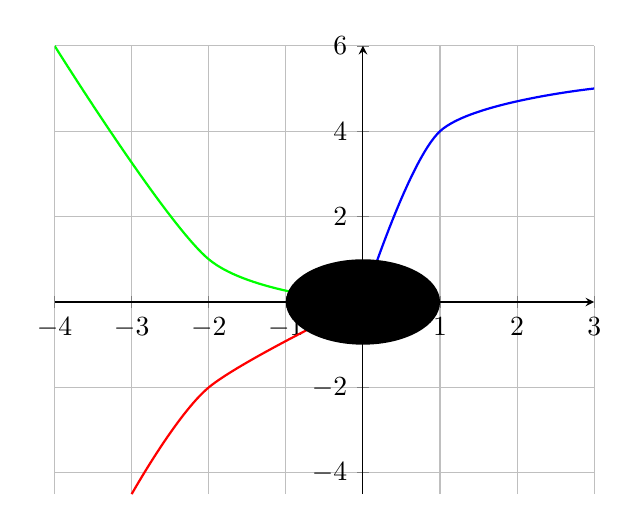
\begin{tikzpicture}
\begin{axis}[grid=major,axis x line=middle,
             axis y line=middle,
             after end axis/.code={
  }]

\addplot[color = green, smooth, thick,] coordinates
    {(-4,6) (-2,1) (0,0)};
\addplot[color = blue, smooth, thick] coordinates
    {(3,5) (1,4) (0,0)};
\addplot[color = red, smooth, thick] coordinates
    {(-3,-4.5) (-2,-2) (0,0)};
\fill[black] (axis cs:0,0) circle (1);
\end{axis}
\end{tikzpicture}
\end{figure}

In the case of $|a| < |b|$, points will move asymptotically towards $R = -J$ and $R = J$. \\
In the case of $|a| = |b|$, points will cycle around the origin infinitely.
\newpage

\subsection{Supremum and Infimum of a Set $\mathcal{A} \subseteq \mathbb{R}$}
\begin{itemize}
\item If $\mathcal{A} \in (-\infty, b]$ for some $b \in \mathbb{R}$, we say $\mathcal{A}$ is bounded above, and that $b$ is an \textbf{upper bound} for $A$. 
\end{itemize}

\begin{theorem}[Supremum Theorem]
If $\mathcal{A} \in \mathbb{R}$, $A \neq \emptyset$, and $A \subseteq (-\infty, b]$ for some $b \in \mathbb{R}$, then there exists $a \in \mathbb{R}$ such that $\mathcal{A} \subseteq (-\infty, a ]$ but if $x < a$, then $\mathcal{A} \not \subseteq (-\infty, x]$. \\
We write $a = \sup{\mathcal{A}}$, call it the \textbf{supremum} of $\mathcal{A}$.
\end{theorem}

Why is this necessary? Consider the set $\mathcal{A} = \{-\frac{1}{n} | n \in \mathbb{N} \}$. It does not have a maximum persay, but it has a supremum $\sup{\mathcal{A}} = 0$. \\ \\
Consider this example: What is $\sup{(-\mathbb{N})}$? It is -1, which also happens to be the maximum of the set.

\begin{theorem}
If max $A$ exists as a real number, then $\sup{A} = \max{A}$.
\end{theorem}

But to answer all these questions, we need to figure out: what exactly are the real numbers? 

\subsection{What is $\mathbb{R}$?}
Let $x = (s,N,d_1,d_2,d_3,\dots,d_k,\dots)$, where:
\begin{itemize}
\item $s \in \{+1,-1\}$
\item $N \in \mathbb{Z}$
\item $d_k \in \mathbb{D} = \{0,1,2,3,4,5,6,7,8,9\}$
\item $\neg (\exists k : d_{k+1} = d_{k+2} = \dots = 0)$, this is to prevent multiple sequences from being the same number
\end{itemize}

In this case, ``2.49'' is shorthand for $(+1,2,4,8,9,9,9,\dots)$

\section{2/4/16}
\textbf{Aim}: Background in $\mathbb{R}$; Fundamental Existence/Uniqueness Question \\

Recall:
\begin{theorem}[Supremum/Infimum Theorem] 
\
\begin{enumerate}
\item If $\mathcal{A}$ is a non-empty set of $\mathbb{R}$, and is bounded above (i.e. $\mathcal \subseteq (-\infty, b]$ for some $b \in \mathbb{R}$), then there is a \underline{least} upper bound for $\mathcal{A}$, namely $a \in \mathbb{R}$ such that
\begin{enumerate}
\item $\mathcal{A} \subseteq (-\infty, a]$
\item if $x < a$, then $\mathcal{A} \not \subseteq (-\infty, x]$
\end{enumerate}
This $a$ is called the called the \textbf{supremum} of $\mathcal{A}$, written $\sup{A}$.
\item $\inf{A}$. This is the \underline{greatest lower bound} for $\mathcal{A}$, or the \textbf{infimum}, provided $\mathcal{A} \neq \emptyset$ and $\mathcal{A}$ has a lower bound at all.
\end{enumerate}
\end{theorem}

Recall that the Riemann integral is taking the limit of a partition over an interval $[a,b]$. But when we take the limit, we make the mesh of the partition, $\norm{\mathcal{P}}$, approach zero, where \[ \mathcal{P} = \max_{1 \le i \le n}{\Delta x_i} \]

To fix this, we can define: \[ \lowint_a^b f(x) \ dx = \sup\left\{ \sum_{i=1}^n[\inf\{f(x) \ | \ x_{i-1} \le x \le x_i \}\Delta x_i] \ |\ a = x_0 < x_1 < \dots < x_n = b\right\} \] % HOW DO YOU TYPE AN INTEGRAL WITH AN UNDERLINE

This is a ``down-and-up'' procedure. The sum of the rectangle areas is a down approximation since we use the minimum possible height to find the area. Then, we take the supremum of that, since for any lower approximation there will always be a higher approximation. Turns out there will never be a maximum; that's why we take the supremum. This is a \textbf{lower Riemann sum}

We can also define the same thing for an \textbf{upper Riemann sum}: \[ \upint_a^b f(x) \ dx = \inf\left\{ \sum_{i=1}^n[\sup\{f(x) \ | \ x_{i-1} \le x \le x_i \}\Delta x_i] \ |\ a = x_0 < x_1 < \dots < x_n = b\right\} \]

Therefore, the following inequality is true: \[ \lowint_a^b f \le \upint_a^b f \]

If these two are equal, then we say that $f$ is \textbf{Riemann integrable}. \\ \\

Here's an example of a function that is NOT Riemann integrable:
\[ f(x) = 
\begin{cases}
0 \text{ if } x \in \mathbb{Q} \cap [0,1] \\
1 \text{ if } x \in [0,1]\backslash \mathbb{Q}
\end{cases}
\]

Note that $\lowint_0^1 f = 0$ and $\upint_0^1 f = 1$, so this is not Riemann integrable.

\subsection{Real Numbers, Again}
We have shorthand for our previous definition of the real numbers.
\[ \mathbb{R} = \{0\} \cup \{(s,N,d_1,d_2,\dots, d_k,\dots \ | \ s \in \{-1,+1\}, N \in \mathbb{Z}^+, d_k \in \mathbb{D}, \text{no 0-tail} \}\]
and the positive reals: \[ \mathbb{R}^+ = \{(s,N,d_1,d_2,\dots) \ | \ s = +1\} \]
Let us write  $x = \underline{N}.\underline{d_1d_2d_3\dots}$ and $y = \underline{M}.\underline{e_1e_2e_3\dots}$. \\ \\
We also define negation as: \[ -(s,N,d_1,d_2,\dots) = (-s,N,d_1,d_2,\dots) \]
Then we can define the ``less than'' operation as follows:
\begin{itemize}
\item If $x,y \in \mathbb{R}^+$, then $x<y$ if either $N < M$ or $N =M$ and $d_1 < e_1$ or $N = M$, $d_1 = e_1$ and $d_2 < e_2$, or...
\item $0<x$ if $x \in \mathbb{R}^+$
\item $x < 0$ if $x \in \mathbb{R}^+$
\item  $x<y$ if $x \in \mathbb{R}^-, y \in \mathbb{R}^+$. 
\item $x,y \in \mathbb{R}^-$, and $x<y$ if $-y < -x$
\end{itemize}





\end{document}
